\documentclass[11pt,a4paper]{article}

\usepackage[margin=1.0in]{geometry}
\usepackage[T1]{fontenc}
\usepackage[utf8]{inputenc}
\usepackage{lmodern}
\usepackage{microtype}
\usepackage{amsmath,amssymb,amsthm,mathtools}
\usepackage{booktabs}
\usepackage{graphicx}
\usepackage{xcolor}
\usepackage{enumitem}
\usepackage{hyperref}

\hypersetup{
  colorlinks=true,
  linkcolor=blue!60!black,
  citecolor=green!45!black,
  urlcolor=blue!65!black,
  pdftitle={Exact Sharp Thresholds, Piecewise-Algebraic Squaring Laws, and Machine-Checked Thermodynamic Mass-Gap Certificates for the Reflection-Positive Purity Bootstrap},
  pdfauthor={Antigravity Frontier Research Agent}
}

\newtheorem{theorem}{Theorem}[section]
\newtheorem{proposition}[theorem]{Proposition}
\newtheorem{lemma}[theorem]{Lemma}
\newtheorem{corollary}[theorem]{Corollary}
\theoremstyle{definition}
\newtheorem{definition}[theorem]{Definition}
\newtheorem{remark}[theorem]{Remark}

\newcommand{\R}{\mathbb{R}}
\newcommand{\Q}{\mathbb{Q}}
\newcommand{\N}{\mathbb{N}}
\newcommand{\Z}{\mathbb{Z}}
\newcommand{\Tr}{\operatorname{Tr}}
\newcommand{\Bgap}{\mathcal{B}_{\mathrm{gap}}}

\title{\textbf{Exact Sharp Thresholds, Piecewise-Algebraic Squaring Laws, and Machine-Checked Thermodynamic Mass-Gap Certificates for the Reflection-Positive Purity Bootstrap}}

\author{Antigravity Frontier Research Agent\thanks{Autonomous scientific research conducted under the \texttt{AIRR-INDEPENDENT-AGENT-1.0} protocol in the computational workspace of Lluis Eriksson. All zero-dependency Lean~4 proofs, exact rational ($\Q$) certificate verifiers, numerical benchmarks, and reproducible scripts are publicly archived at \url{https://github.com/lluiseriksson/sharp-purity-bootstrap}.}}

\date{November 24, 2026}

\begin{document}
\maketitle

\begin{abstract}
The reflection-positive purity bootstrap introduced for the Haldane-gap proof~\cite{OpenAI2026Haldane,Tasaki2026Purity} and extended to higher dimensions, quasi-degenerate ground states, fermions, and tensor networks by Grover~\cite{Grover2026Extensions} certifies a thermodynamic-limit spectral gap $\Delta_\infty > 0$ from finite-size Euclidean partition-function purities $S$ and $T$. Existing analyses rely on conservative defect cutoffs ($u \le 0.01$ in $d=1$ and $1 - Q \le 1/(2a^2)$ in $d$ spatial dimensions with $a = 2^{d+1}-1$) and yield a flat gap ceiling $\Delta_\infty > (\log 2)/\beta_0$ insensitive to the actual purity margin. Here we derive the \emph{exact} extremal laws and sharp stability boundaries of the purity bootstrap in arbitrary dimension $d \ge 1$ and build a machine-checked, zero-floating-point-trust certification pipeline. First, we solve the simplex squaring minimization problem $\inf\{\sum w_i^4 / (\sum w_i^2)^2 : w_i \ge 0,\ \sum w_i = 1,\ \sum w_i^2 = p\}$ in closed piecewise-algebraic form on all of $(0,1]$; on $(1/2,1]$ it collapses to $h_1^*(p) = 1 - (1-p)^2/(2p^2)$ via a three-line pure ring-algebra proof, accompanied by the uniquely attained spectral-gap enclosure $e^{\beta \Delta} \ge (1+\sqrt{2p-1})^2/(2(1-p))$. Second, exploiting the exact staggered space-time plaquette identity in a cyclic Gauss--Seidel recurrence, we derive the algebraic uniform threshold $p_c(d) = 1 - u_c^*(d)$ solving $2p^{2a} = (1-p)(\sum_{j=0}^{a-1} p^j)^2$, widening the 1D uniform basin by $12.73\times$ ($u_c^*(1) = 0.127311$) and enlarging the single-ratio $Q$ threshold by $3.26\times$ to $7.63\times$ across $d = 1,\dots,5$ (asymptotically $8\times$, scaling as $4/(a(a+1))$ vs.\ $1/(2a^2)$). Third, we prove an exact doubly-exponential contraction bound yielding $\Delta_\infty \ge \frac{1}{2^N \beta_0}\log(1/(K_d(u_N)u_N))$ for \emph{all} intervening even hypercube lengths $\ell \ge L_0$, breaking the $(\log 2)/\beta_0$ ceiling by arbitrarily large factors. We formalize all 16 core algebraic theorems and lemmas in zero-dependency Lean~4 (\texttt{v4.35.0}, zero \texttt{sorry}, zero \texttt{Classical.choice}), verify rational logarithm mass-gap bounds strictly over $\Q$, and benchmark across the 1D transverse-field Ising model ($2.24\times$--$4.72\times$ closer to $h_c=1$, up to $9.03\times$ tighter gaps), the $g=2$ ferromagnetic phase via exact Kramers--Wannier sector duality, 2D ($D=3$) lattices, and synthetic noisy intervals (0 false certifications across 200 critical and 200 near-boundary trials). On interacting spin chains, we prove an $\mathfrak{su}(3)$ determinant obstruction showing that the Spin-1 AKLT chain violates bond-reflection positivity for every $U \in U(3)$, and certify exact-$\Q$ thermodynamic gaps on two provably bond-reflection-positive non-integrable chains—Spin-1 Heisenberg with single-ion anisotropy ($L_0=4 \to 8$) and Spin-1/2 dimerized Heisenberg ($L_0=6 \to 12$)—where Grover's $u \le 0.01$ fails at every tested parameter.
\end{abstract}

\section{Introduction}
\label{sec:intro}

Establishing a uniform spectral gap $\Delta_\infty = \liminf_{L\to\infty}(E_1(L)-E_0(L)) > 0$ in the thermodynamic limit of interacting quantum many-body lattice Hamiltonians is a central open problem in mathematical physics~\cite{Haldane1983Continuum,Haldane1983Nonlinear,Affleck1987AKLT,Affleck1988AKLT}. Classical finite-size criteria such as Knabe's bound~\cite{Knabe1988Energy} and its modern refinements~\cite{Gosset2016Local,Lemm2019Spectral,Anshu2020Improved} require the Hamiltonian to be frustration-free, excluding generic frustrated or non-commuting models such as the spin-$1$ Heisenberg antiferromagnet.

A recent breakthrough—the \emph{reflection-positive purity bootstrap}~\cite{OpenAI2026Haldane,Tasaki2026Purity}—circumvents frustration-freeness by exploiting Osterwalder--Schrader reflection positivity~\cite{Osterwalder1973Axioms,Frohlich1978Reflection} of the Euclidean partition function $Z(L_1,\dots,L_d;\beta) = \Tr(e^{-\beta H_{L_1,\dots,L_d}})$. Writing normalized partition-function ratios (``purities'') in spatial and temporal directions,
\begin{equation}
  S(L,\beta) \coloneqq \frac{Z(2L,\beta)}{Z(L,\beta)^2}, \qquad
  T(L,\beta) \coloneqq \frac{Z(L,2\beta)}{Z(L,\beta)^2},
  \label{eq:ST_def}
\end{equation}
reflection positivity ensures that both $S(L,\beta) = \sum_i w_i^2 / (\sum_i w_i)^2$ (for the spatial transfer operator) and $T(L,\beta)$ (for the Gibbs transfer operator $e^{-\beta H_L}$) are purities of nonnegative probability distributions $w = (w_i)$ on the unit simplex, hence lie in $(0,1]$. Doubling along an axis squares the underlying spectrum ($w_i \mapsto w_i^2$), driving the purity closer to $1$, while passing across orthogonal axes incurs a plaquette penalty. Grover~\cite{Grover2026Extensions} systematically generalized this bootstrap to arbitrary spatial dimension $d \ge 1$ ($D = d+1$ space-time axes), quasi-degenerate ground states ($g \ge 2$), fermionic parity sectors, and tensor-network states.

Despite its elegance, the current purity bootstrap suffers from four structural bottlenecks that severely limit practical certification on finite lattices:
\begin{enumerate}[leftmargin=1.6em,itemsep=2pt]
  \item \textbf{Loose squaring and gap-from-purity inequalities.} Prior bounds use suboptimal lower envelopes for $\sum w_i^4 / (\sum w_i^2)^2$ and for the gap ratio $w_0/w_1$, losing a factor of up to $2$ in the purity defect at every doubling step.
  \item \textbf{Conservative multi-axis thresholds.} Grover~\cite{Grover2026Extensions} requires $u \le 0.01$ in $d=1$ and $1 - Q \le 1/(2a^2)$ in $d$ spatial dimensions (where $a = 2^{d+1}-1$), discarding over $90\%$ of the true certifiable region in 1D and a factor of up to $8\times$ in higher dimensions due to simultaneous (Jacobi) rather than sequential (Gauss--Seidel) multi-axis updates.
  \item \textbf{Flat thermodynamic gap ceiling.} Because existing proofs terminate once $T(L,\beta)$ crosses a fixed constant, they produce the flat bound $\Delta_\infty > (\log 2)/\beta_0$, which actually \emph{degrades} as $1/\beta_0$ when one lowers temperature to enter the bootstrap basin—even when the initial purity defect is $10^{-6}$!
  \item \textbf{Unverified floating-point and finite-sample certification.} Numerical partition functions from exact diagonalization, tensor networks, or Monte Carlo carry floating-point rounding or statistical error; without monotone interval propagation and exact rational verification, a near-boundary rounding error could falsely certify a gapless critical point.
\end{enumerate}

\paragraph{Summary of Contributions.}
We resolve all four bottlenecks with exact extremal mathematics, zero-dependency Lean~4 machine verification, and exact-$\Q$ numerical certificates:
\begin{itemize}[leftmargin=1.6em,itemsep=2pt]
  \item \textbf{Exact Piecewise-Algebraic Squaring Law \& Gap Enclosures (Section~\ref{sec:squaring}):} Theorem~\ref{thm:squaring_general} characterizes the global infimum $h^*(p) = \inf\{\sum w_i^4 / (\sum w_i^2)^2 : \sum w_i = 1,\ \sum w_i^2 = p\}$ across all $p \in (0,1]$; on $(1/2,1]$, it coincides with the rational envelope $h_1^*(p) = 1 - (1-p)^2/(2p^2)$, which admits a purely algebraic three-line proof (Theorem~\ref{thm:squaring_k1}). Theorem~\ref{thm:gap_from_purity} establishes the uniquely sharp spectral-gap ratio $w_0/w_1 \ge (1+\sqrt{2p-1})^2/(2(1-p))$.
  \item \textbf{Exact $D$-Dimensional Cyclic Gauss--Seidel Thresholds (Section~\ref{sec:thresholds}):} Leveraging the exact staggered space-time plaquette identity in a cyclic Gauss--Seidel iteration (Theorem~\ref{thm:gs_1d}), we prove that the uniform stability boundary $p_c(d) = 1 - u_c^*(d)$ is the unique root in $(1/2,1)$ of $2p^{2a} = (1-p)(\sum_{j=0}^{a-1} p^j)^2$, yielding $u_c^*(1) = 0.127311$ ($12.73\times$ vs.\ $0.01$). For the single-ratio hypercube invariant $Q$, eliminating redundant leading-axis factors yields Theorem~\ref{thm:hypercube_Q}, improving $1 - Q_c^*(d)$ by $3.26\times$ to $7.63\times$ for $d=1,\dots,5$ and asymptotically $8\times$ ($4/(a(a+1))$ vs.\ $1/(2a^2)$).
  \item \textbf{Unbounded Asymptotic Gap Bounds \& Intervening Lengths (Section~\ref{sec:asymptotic}):} Theorem~\ref{thm:doubly_exp} proves explicit doubly-exponential decay $K_d u_{N+m} \le (K_d u_N)^{2^m}$, certifying $\Delta_\infty \ge \frac{1}{2^N \beta_0}\log(1/(K_d(u_N)u_N))$—scaling as $\Omega(\log(1/u_0)/\beta_0)$ and breaking the $(\log 2)/\beta_0$ ceiling. Theorem~\ref{thm:intervening} and Proposition~\ref{prop:intervening_d} transfer this exact lower bound from dyadic lengths $2^n L_0$ to \emph{every} intervening even hypercube length $\ell \ge L_0$, and Corollary~\ref{cor:z2_ferro} handles the ferromagnetic 1D TFIM via exact Kramers--Wannier sector duality.
  \item \textbf{Machine-Checked Lean~4 Formalization, Exact-$\Q$ Verifier \& Bond-RP Benchmarks (Sections~\ref{sec:formalization}--\ref{sec:experiments}):} All 16 core algebraic theorems and lemmas listed in Table~\ref{tab:lean_manifest} are formalized in zero-dependency Lean~4 (\texttt{v4.35.0}, 0 \texttt{sorry}, 0 \texttt{Classical.choice}). Theorem~\ref{thm:interval_mono} guarantees fail-closed finite-sample interval propagation and sound downward-quantized $\Q$-certification including exact rational logarithm bounds. We benchmark the pipeline on the 1D TFIM, prove an $\mathfrak{su}(3)$ determinant no-go obstruction for bond-RP of the Spin-1 AKLT chain, and certify exact-$\Q$ gaps on two genuinely bond-RP non-integrable spin chains (Spin-1 Heisenberg+$D$ and Spin-1/2 dimerized Heisenberg), plus 2D ($D=3$) lattices and synthetic noisy intervals.
\end{itemize}

\section{Exact Piecewise-Algebraic Squaring Law and Gap Enclosures}
\label{sec:squaring}

Let $\Delta_\infty^+ \coloneqq \{w = (w_i)_{i \ge 0} : w_i \ge 0,\ \sum_i w_i = 1\}$ denote the countable probability simplex (for finite transfer matrices, all but finitely many $w_i$ vanish), with purity $p(w) \coloneqq \sum_i w_i^2 \in (0,1]$ and fourth moment $q(w) \coloneqq \sum_i w_i^4$. Under one axis doubling, the normalized weights transform as $w_i \mapsto w_i^2 / p(w)$, so the doubled purity is $p'(w) = q(w) / p(w)^2$.

\begin{theorem}[Exact Piecewise-Algebraic Squaring Law on ${(0,1]}$]
\label{thm:squaring_general}
For every $p \in (0,1]$, let $k = \lfloor 1/p \rfloor \in \N_{\ge 1}$ so that $p \in \bigl(\tfrac{1}{k+1}, \tfrac{1}{k}\bigr]$, and define
\begin{equation}
  a_k(p) \coloneqq \frac{k + \sqrt{k((k+1)p - 1)}}{k(k+1)}, \qquad
  b_k(p) \coloneqq \frac{1 - \sqrt{k((k+1)p - 1)}}{k+1}.
  \label{eq:ak_bk}
\end{equation}
Then over all probability distributions $w \in \Delta_\infty^+$ satisfying $\sum_i w_i^2 = p$,
\begin{equation}
  \inf_{\substack{w \in \Delta_\infty^+ \\ \sum w_i^2 = p}} \frac{\sum_i w_i^4}{p^2}
  \;=\; h^*(p) \;\coloneqq\; \frac{k\, a_k(p)^4 + b_k(p)^4}{p^2},
  \label{eq:hstar_general}
\end{equation}
and the infimum is uniquely attained (up to permutation and zero padding) by the $(k+1)$-point spectrum $w^* = (\underbrace{a_k(p),\dots,a_k(p)}_{k\text{ times}}, b_k(p), 0, 0, \dots)$.
\end{theorem}

\begin{proof}
Fix $p \in (0,1]$ and consider minimizing $f(w) = \sum_{i=1}^m w_i^4$ over the compact set $K_m(p) = \{w \in \R_{\ge 0}^m : \sum_i w_i = 1,\ \sum_i w_i^2 = p\}$ for arbitrary $m \ge k+1$. First, if all positive coordinates of a minimizer $w$ are equal ($w_i = 1/r$ on its support of size $r$), then $p = 1/r$ is an exact reciprocal integer ($r = k$) and Cauchy--Schwarz gives $\sum w_i^4 \ge (\sum w_i^2)^2/r = p^3 = k(1/k)^4$, matching~\eqref{eq:hstar_general} with $b_k(1/k) = 0$. Otherwise, $w$ has at least two distinct positive coordinates, so the gradients $(1,\dots,1)$ and $(2w_1,\dots,2w_m)$ are linearly independent on the positive support (LICQ holds). By Karush--Kuhn--Tucker stationarity, $w$ admits multipliers $\lambda, \mu \in \R$ such that every positive coordinate $w_i > 0$ satisfies the depressed cubic
\begin{equation}
  g(w_i) \;\coloneqq\; 4 w_i^3 - 2\mu w_i - \lambda \;=\; 0.
  \label{eq:kkt_cubic}
\end{equation}
Since a depressed cubic has at most two positive roots, every positive coordinate of $w$ takes at most two distinct values $a > b > 0$. By Rolle's theorem on $g(x) = 4x^3 - 2\mu x - \lambda$ (whose derivative $g'(x) = 12x^2 - 2\mu$ has a single positive zero), we have $g'(a) = 12a^2 - 2\mu > 0$ and $g'(b) = 12b^2 - 2\mu < 0$. If $w$ contained $s \ge 2$ copies of $b$, then the perturbation vector $\delta$ with $(+1, -1)$ on two $b$-coordinates and $0$ elsewhere lies in the tangent subspace $\{\delta : \sum \delta_i = 0,\ \sum w_i \delta_i = 0\}$ of both equality constraints; by LICQ, the second-order necessary condition requires the Lagrangian Hessian form $\sum_i (12 w_i^2 - 2\mu)\delta_i^2 = 2(12b^2 - 2\mu) \ge 0$, contradicting $g'(b) < 0$. Hence $s \le 1$, so any minimizer has support $(\underbrace{a,\dots,a}_{r}, b)$ with $a \ge b \ge 0$.

Eliminating $b = 1 - r a$ from $r a^2 + b^2 = p$ gives $r(r+1)a^2 - 2ra + (1-p) = 0$. Positivity of $b = 1 - ra \ge 0$ forces $1/p \ge r$ (with $r = 1/p$ when $b=0$), while real roots require $r((r+1)p - 1) \ge 0$, i.e., $r \ge \lceil 1/p \rceil - 1$. For non-integer $1/p$ this uniquely selects $r = k = \lfloor 1/p \rfloor$, and for integer $1/p = k$ the boundary value $b=0$ agrees continuously with $r = k-1$ at $a = b = 1/k$. Taking the larger root $a \ge b$ yields~\eqref{eq:ak_bk}. Since this lower bound is independent of $m$, passing to $m \to \infty$ proves~\eqref{eq:hstar_general} over all of $\Delta_\infty^+$; moreover, uniqueness on $\Delta_\infty^+$ follows because any minimizer $w \in \Delta_\infty^+$ with three distinct positive coordinates (or two copies of a non-maximal positive value) would violate the finite-support KKT conditions when fixing all remaining coordinates.
\end{proof}

When $p \in (1/2, 1]$ ($k = 1$), the square roots in~\eqref{eq:ak_bk} cancel identically, yielding a rational lower-bound envelope $h_1^*(p)$ that coincides with $h^*(p)$ on $(1/2,1]$ and admits a three-line elementary proof requiring no calculus (formalized over arbitrary ordered fields in Lean~4; see Table~\ref{tab:lean_manifest}).

\begin{theorem}[Three-Line Algebraic Squaring Law on ${(1/2, 1]}$]
\label{thm:squaring_k1}
For every finite or countable distribution $w \in \Delta_\infty^+$ with purity $p = \sum_i w_i^2 > 0$,
\begin{equation}
  \sum_i w_i^4 \;\ge\; p^2 - \frac{(1 - p)^2}{2},
  \qquad\text{equivalently}\qquad
  \frac{\sum_i w_i^4}{p^2} \;\ge\; h_1^*(p) \;\coloneqq\; 1 - \frac{(1 - p)^2}{2 p^2}.
  \label{eq:hstar_k1}
\end{equation}
Moreover: (i) $h_1^*(p) = h^*(p)$ for all $p \in (1/2, 1]$ and equality holds identically on every two-level spectrum $(a, 1-a)$; (ii) $h_1^*(p)$ is strictly increasing on $(0, 1]$; and (iii) writing $u = 1 - p$, the defect contracts quadratically as $1 - h_1^*(1 - u) = \frac{u^2}{2(1-u)^2}$.
\end{theorem}

\begin{proof}
Let $P_1 \coloneqq \sum_{i < j} w_i w_j$ and $P_2 \coloneqq \sum_{i < j} (w_i w_j)^2$. Expanding $(\sum_i w_i)^2 = 1$ and $(\sum_i w_i^2)^2 = p^2$ yields the two exact identities
\[
  1 - p = 2 P_1, \qquad p^2 - \sum_i w_i^4 = 2 P_2.
\]
Since every term $w_i w_j \ge 0$, we have $P_2 = \sum_{i<j}(w_i w_j)^2 \le \bigl(\sum_{i<j} w_i w_j\bigr)^2 = P_1^2 = (1-p)^2/4$, with equality whenever at most one pair $(i,j)$ is nonzero (i.e., any two-level spectrum). Multiplying by $2$ gives $p^2 - \sum_i w_i^4 \le (1-p)^2/2$, which rearranges immediately to~\eqref{eq:hstar_k1}. Monotonicity of $h_1^*(p)$ on $(0,1]$ follows since $(1-p)/p = p^{-1}-1$ is strictly decreasing and nonnegative.
\end{proof}

Notice that $h_1^*(p)$ provides a valid lower bound for \emph{all} $p \in (0,1]$ (though it is sharp only on $(1/2, 1]$, where it agrees with $h^*(p)$, and becomes nonpositive below $p = \sqrt{2}-1 \approx 0.414$). Compared to naive bounds of the form $1 - u' \ge 1 - u^2/(1-u)^2$ or linear defect relaxations, the exact factor of $\frac{1}{2}$ in $1 - h_1^*(1-u) = \frac{u^2}{2(1-u)^2}$ doubles the permissible defect at every single step. For brevity, we write $h^*(p) = h_1^*(p)$ throughout Sections~\ref{sec:thresholds}--\ref{sec:formalization}, where all intermediate purities lie strictly in $(1/2, 1]$.

We next derive the exact sharp extraction of the spectral gap $\Delta = E_1 - E_0$ from a Gibbs purity $p = T(L,\beta) = \sum_i w_i^2$ where $w_i = e^{-\beta E_i}/Z(L,\beta)$ are sorted $w_0 \ge w_1 \ge \cdots \ge 0$.

\begin{theorem}[Sharp Gap-from-Purity and Tail-Mass Enclosures]
\label{thm:gap_from_purity}
Let $w \in \Delta_\infty^+$ with $w_0 \ge w_1 \ge \cdots \ge 0$ and purity $p = \sum_{i \ge 0} w_i^2$. Then:
\begin{enumerate}[label=(\alph*),leftmargin=2em,itemsep=2pt]
  \item $w_0 \ge p$ and $1 - p \ge 2 w_0 (1 - w_0)$, hence $(2w_0 - 1)^2 \ge 2p - 1$. In particular, for $p \in (1/2, 1]$,
  \begin{equation}
    w_0 \;\ge\; \frac{1 + \sqrt{2p - 1}}{2}, \qquad
    \sum_{i \ge 1} w_i \;=\; 1 - w_0 \;\le\; \frac{1 - \sqrt{2p - 1}}{2}.
    \label{eq:sharp_w0}
  \end{equation}
  \item If $p \in (1/2, 1)$ and $w_1 > 0$, then
  \begin{equation}
    e^{\beta \Delta} \;=\; \frac{w_0}{w_1} \;\ge\; \frac{2 w_0^2}{1 - p} \;\ge\; \frac{(1 + \sqrt{2p - 1})^2}{2(1 - p)}.
    \label{eq:sharp_gap_ratio}
  \end{equation}
  Every inequality in~\eqref{eq:sharp_w0}--\eqref{eq:sharp_gap_ratio} is attained with exact equality on two-level spectra $(w_0, 1-w_0)$.
\end{enumerate}
\end{theorem}

\begin{proof}
Since $w_i \le w_0$ for all $i \ge 1$, $p = w_0^2 + \sum_{i\ge 1} w_i^2 \le w_0(w_0 + \sum_{i\ge 1} w_i) = w_0$. Next, $\sum_{i \ge 1} w_i^2 \le (\sum_{i\ge 1} w_i)^2 = (1 - w_0)^2$, so $p \le w_0^2 + (1-w_0)^2 = 1 - 2w_0(1-w_0)$, giving $1 - p \ge 2 w_0 (1-w_0)$. Multiplying by $2$ and subtracting from $1$ yields $(2w_0-1)^2 = 1 - 4w_0(1-w_0) \ge 2p - 1$. Since $w_0 \ge p > 1/2$, taking the positive square root gives~\eqref{eq:sharp_w0}. Finally, $w_1 \le 1 - w_0$ implies $2 w_0 w_1 \le 2 w_0 (1 - w_0) \le 1 - p$, so dividing by $w_1(1-p)/w_0 > 0$ gives $w_0 / w_1 \ge 2 w_0^2 / (1-p)$, and substituting~\eqref{eq:sharp_w0} gives~\eqref{eq:sharp_gap_ratio}.
\end{proof}

As $p \to 1^-$,~\eqref{eq:sharp_gap_ratio} gives $w_0/w_1 \ge \frac{2}{1-p}(1 - O(1-p))$, which is asymptotically $2\times$ tighter in the ratio (an additive $+(\log 2)/\beta$ improvement in $\Delta$) than the elementary bound $w_0/w_1 \ge p/(1-p)$ and exact on two-level spectra. All four algebraic core lemmas of Theorem~\ref{thm:gap_from_purity} are Lean-verified (Table~\ref{tab:lean_manifest}).

\section{Cyclic Gauss--Seidel Recurrence and Sharp \texorpdfstring{$D$}{D}-Dimensional Thresholds}
\label{sec:thresholds}

\subsection{Exact Space-Time Plaquette Identity and 1D Cyclic Gauss--Seidel Bootstrap}

Consider a reflection-positive 1D quantum lattice Hamiltonian with Euclidean partition functions $Z(L,\beta) > 0$ for even lengths $L$ and $\beta > 0$, with spatial purity $S(L,\beta) = Z(2L,\beta)/Z(L,\beta)^2 \in (0,1]$ and temporal purity $T(L,\beta) = Z(L,2\beta)/Z(L,\beta)^2 \in (0,1]$. On any elementary space-time plaquette $(L,\beta) \to (2L,2\beta)$, direct algebraic cancellation (Lean: \texttt{plaquette\_exact\_identity}) gives the exact identity
\begin{equation}
  S(L, 2\beta)\, T(L,\beta)^2 \;=\; \frac{Z(2L, 2\beta)}{Z(L,\beta)^4} \;=\; T(2L, \beta)\, S(L,\beta)^2.
  \label{eq:plaquette_id}
\end{equation}
Because $T(L,\beta) \le 1$ by reflection positivity,~\eqref{eq:plaquette_id} immediately yields the sharp plaquette transfer inequality (Lean: \texttt{plaquette\_lower\_bound})
\begin{equation}
  S(L, 2\beta) \;\ge\; S(L,\beta)^2\, T(2L,\beta).
  \label{eq:plaquette_lb}
\end{equation}
Crucially, note that $S(L,2\beta)$ does \emph{not} satisfy $S(L,2\beta) \ge S(L,\beta)^2$ in general (we verified counterexamples with $S(L,2\beta)/S(L,\beta)^2 \approx 0.981 < 1$ on reflection-positive two-mode transfer matrices); the factor $T(2L,\beta)$ in~\eqref{eq:plaquette_lb} is sharp and indispensable.

Now define the diagonalized scale-doubled sequence
\[
  S_n \coloneqq S(2^n L_0, 2^n \beta_0), \qquad T_n \coloneqq T(2^{n+1} L_0, 2^n \beta_0), \qquad n \ge 0.
\]
Applying~\eqref{eq:plaquette_lb} to $(2^n L_0, 2^n \beta_0)$ yields $S(2^n L_0, 2^{n+1}\beta_0) \ge S_n^2 T_n$. Doubling the spatial axis from $2^n L_0$ to $2^{n+1} L_0$ at fixed $2^{n+1}\beta_0$ squares the spatial transfer-matrix spectrum, so by Theorem~\ref{thm:squaring_k1} and monotonicity of $h^*$:
\begin{equation}
  S_{n+1} \;=\; S(2^{n+1} L_0, 2^{n+1}\beta_0) \;\ge\; h^*\!\bigl(S(2^n L_0, 2^{n+1}\beta_0)\bigr) \;\ge\; h^*(S_n^2 T_n).
  \label{eq:gs_1d_S}
\end{equation}
Next, applying the transposed plaquette identity to $(2^{n+1}L_0, 2^n \beta_0)$ uses the \emph{already-updated} spatial purity $S_{n+1}$:
\[
  T(2^{n+2}L_0, 2^n \beta_0) \;=\; \frac{T_n^2\, S_{n+1}}{S(2^{n+1}L_0, 2^n \beta_0)^2} \;\ge\; T_n^2 S_{n+1}.
\]
Doubling the temporal axis from $2^n \beta_0$ to $2^{n+1}\beta_0$ at fixed length $2^{n+2}L_0$ squares the Gibbs spectrum, yielding the exact \emph{cyclic Gauss--Seidel} update:
\begin{equation}
  T_{n+1} \;=\; T(2^{n+2}L_0, 2^{n+1}\beta_0) \;\ge\; h^*(T_n^2 S_{n+1}).
  \label{eq:gs_1d_T}
\end{equation}

\begin{theorem}[1D Cyclic Gauss--Seidel Bootstrap and Exact Uniform Threshold]
\label{thm:gs_1d}
Define $\Phi_{\mathrm{GS}}^{(1)}(s,t) = \bigl(h^*(s^2 t),\; h^*(t^2 h^*(s^2 t))\bigr)$.
\begin{enumerate}[label=(\alph*),leftmargin=2em,itemsep=2pt]
  \item \textbf{Inductive Soundness \& Monotonicity (Table~\ref{tab:lean_manifest}).} If $0 < s_0 \le S_0$ and $0 < t_0 \le T_0$, and every iterate $(s_k, t_k) = (\Phi_{\mathrm{GS}}^{(1)})^k(s_0, t_0)$ for $k \le N$ remains strictly positive with intermediate products in $(0,1]$, then $s_k \le S_k$ and $t_k \le T_k$ for all $k \le N$.
  \item \textbf{Exact Uniform Stability Threshold.} Along the symmetric diagonal $s_0 = t_0 = p$, the map converges to $(1,1)$ if and only if $p > p_c(1) \coloneqq 1 - u_c^*(1)$, where $p_c(1)$ is the unique root in $(1/2, 1)$ of $h^*(p^3) = p$, equivalently the polynomial equation
  \begin{equation}
    2 p^6 \;=\; (1 - p)\bigl(1 + p + p^2\bigr)^2,
    \label{eq:poly_1d}
  \end{equation}
  giving $p_c(1) = 0.8726892136\dots$ and $u_c^*(1) = 0.1273107864\dots$—a $\mathbf{12.73\times}$ wider uniform threshold than Grover's $u \le 0.01$~\cite{Grover2026Extensions}.
  \item \textbf{Anisotropic Basin.} Even when $s_0 < p_c(1)$, $(s_0, t_0)$ lies in the exact certifiable gapped basin $\Bgap^{(1)}$ whenever $t_0 > t_{\mathrm{crit}}(s_0)$ (e.g., $s_0 = 0.80, t_0 > 0.9675$, or $s_0 = 0.785, t_0 > 0.9950$).
\end{enumerate}
\end{theorem}

\begin{proof}
Part (a) follows by induction from~\eqref{eq:gs_1d_S}--\eqref{eq:gs_1d_T} and monotonicity of $h^*$ on $(0,1]$. For (b), at a fixed point $(p,p)$ of $\Phi_{\mathrm{GS}}^{(1)}$, both coordinates satisfy $p = h^*(p^3) = 1 - (1-p^3)^2 / (2p^6)$. Rearranging $1-p = (1-p)^2(1+p+p^2)^2/(2p^6)$ and cancelling $1-p > 0$ gives~\eqref{eq:poly_1d}. On $(1/2,1)$, the left-hand side $2p^6$ is strictly increasing from $1/32$ to $2$, while $(1-p)(1+p+p^2)^2 = (1-p^3)(1+p+p^2)$ has derivative $-(3p^2)(1+p+p^2) + (1-p^3)(1+2p) < 0$ for all $p \in (0.65, 1)$ (and $2p^6 < (1-p)(1+p+p^2)^2$ on $(1/2, 0.65]$), ensuring a unique root $p_c(1) \approx 0.8726892136$. Since $\Phi_{\mathrm{GS}}^{(1)}$ is componentwise strictly increasing, $p > p_c(1)$ implies $h^*(p^3) > p$, forcing $(s_n, t_n) \uparrow (1,1)$ monotonically.
\end{proof}

\subsection{General \texorpdfstring{$D$}{D}-Dimensional Cyclic Bootstrap and \texorpdfstring{$8\times$}{8x} Single-\texorpdfstring{$Q$}{Q} Improvement}

In $d$ spatial dimensions ($D = d+1$ space-time axes with initial extents $\vec{L}_0 = (L_{0,0},\dots,L_{0,D-1})$ where $L_{0,D-1} = \beta_0$), let $p_k(\vec{L}) \coloneqq Z(\vec{L} + L_k e_k) / Z(\vec{L})^2 \in (0,1]$ denote the axis-$k$ purity at geometry $\vec{L}$. Crucially, to obtain exact telescoping across all $D$ orthogonal axes, we track the \emph{staggered staircase} state vector at doubling scale $n \ge 0$:
\begin{equation}
  p_k^{(n)} \;\coloneqq\; p_k\!\bigl(2^{n+1} L_{0,0},\,\dots,\, 2^{n+1} L_{0,k-1},\; 2^n L_{0,k},\,\dots,\, 2^n L_{0,D-1}\bigr),
  \qquad k = 0,\dots,D-1.
  \label{eq:D_staircase}
\end{equation}
Direct substitution yields the exact $D$-dimensional telescoping hypercube identity
\begin{equation}
  Q^{(n)} \;\coloneqq\; \prod_{j=0}^{D-1} \bigl(p_j^{(n)}\bigr)^{2^{D-1-j}}
  \;=\; \frac{Z(2^{n+1}\vec{L}_0)}{Z(2^n \vec{L}_0)^{2^D}}.
  \label{eq:D_telescope}
\end{equation}
For $k=0$, comparing $Z(2^{n+1}\vec{L}_0)$ along the doubled axis $0$ against $Z(2^{n+1}L_{0,0}, 2^n L_{0,1},\dots,2^n L_{0,D-1})$ via the exact $D$-dimensional plaquette identity gives
\[
  p_0\!\bigl(2^n L_{0,0},\, 2^{n+1} L_{0,1},\,\dots,\, 2^{n+1} L_{0,D-1}\bigr)
  \;\ge\; \frac{Z(2^{n+1}\vec{L}_0)}{Z(2^n \vec{L}_0)^{2^D}}
  \;=\; \prod_{j=0}^{D-1} \bigl(p_j^{(n)}\bigr)^{2^{D-1-j}},
\]
since all denominator purities on the intervening hypercube faces lie in $(0,1]$. Doubling axis $0$ from $2^n L_{0,0}$ to $2^{n+1} L_{0,0}$ then squares the axis-$0$ transfer-matrix spectrum, yielding $p_0^{(n+1)} \ge h^*\bigl(\prod_{j=0}^{D-1} (p_j^{(n)})^{2^{D-1-j}}\bigr)$. Advancing cyclically along axes $k = 0, 1, \dots, D-1$ shifts the staircase window by one axis at each step, yielding the exact cyclic Gauss--Seidel recurrence on $(p_0,\dots,p_{D-1})$:
\begin{equation}
  p_k^{\mathrm{new}} \;=\; h^*\!\Biggl(\,\prod_{j=0}^{D-1} \tilde{p}_{k,j}^{\,2^{D-1-j}}\Biggr), \qquad
  \tilde{p}_{k} = \bigl(p_k,\dots,p_{D-1},\, p_0^{\mathrm{new}},\dots,p_{k-1}^{\mathrm{new}}\bigr),
  \label{eq:D_gs_step}
\end{equation}
where the exponents sum to $a \coloneqq \sum_{j=0}^{D-1} 2^j = 2^D - 1 = 2^{d+1} - 1$.

\begin{theorem}[Sharp $D$-Dimensional Uniform and Single-$Q$ Thresholds]
\label{thm:hypercube_Q}
Let $D = d+1 \ge 2$ and $a = 2^D - 1$.
\begin{enumerate}[label=(\alph*),leftmargin=2em,itemsep=2pt]
  \item \textbf{Exact Uniform Threshold.} A uniform initial staircase $p_0 = \cdots = p_{D-1} = p$ converges to $(1,\dots,1)$ under the cyclic Gauss--Seidel map~\eqref{eq:D_gs_step} if and only if $p > p_c(d) = 1 - u_c^*(d)$, where $p_c(d)$ is the unique root in $(1/2,1)$ of
  \begin{equation}
    2 p^{2a} \;=\; (1 - p)\left(\sum_{j=0}^{a-1} p^j\right)^2,
    \qquad\text{so}\qquad
    u_c^*(d) \;=\; \frac{2}{a^2} + O\!\left(\frac{1}{a^3}\right).
    \label{eq:poly_D}
  \end{equation}
  \item \textbf{Exact Single-$Q$ Contraction and $8\times$ Asymptotic Gain (Table~\ref{tab:lean_manifest}).} For the telescoping hypercube invariant $Q = \prod_{j=0}^{D-1} p_j^{2^{D-1-j}} \in (0,1]$, at step $k \in \{0,\dots,D-1\}$ of~\eqref{eq:D_gs_step} the old trailing product satisfies $\prod_{j=k}^{D-1} p_j^{2^{D-1-j}} \ge Q$, whence raising to $2^k$ yields
  \begin{equation}
    p_k^{\mathrm{new}} \;\ge\; h^*\!\left(Q^{2^k} \prod_{r=0}^{k-1} (p_r^{\mathrm{new}})^{2^{k-1-r}}\right).
    \label{eq:single_Q_gs}
  \end{equation}
  Consequently, $Q^{\mathrm{new}} \ge \Psi_D(Q) \coloneqq \prod_{k=0}^{D-1} (q_k(Q))^{2^{D-1-k}}$, where $q_k(Q)$ is defined recursively by the right-hand side of~\eqref{eq:single_Q_gs}. The exact single-$Q$ stability threshold $1 - Q_c^*(d)$ (unique root of $\Psi_D(Q) = Q$ on the valid domain where all $q_k > 1/2$) satisfies
  \begin{equation}
    1 - Q_c^*(d) \;=\; \frac{4}{a(a+1)} + O\!\left(\frac{1}{a^3}\right)
    \;\sim\; 8 \cdot \frac{1}{2a^2}
    \qquad (d \to \infty),
    \label{eq:single_Q_asymp}
  \end{equation}
  delivering an asymptotic $\mathbf{8\times}$ enlargement over Grover's threshold $1 - Q \le 1/(2a^2)$~\cite{Grover2026Extensions} ($3.26\times$ at $d=1$, $5.28\times$ at $d=2$, $6.56\times$ at $d=3$, $7.26\times$ at $d=4$, $7.63\times$ at $d=5$).
\end{enumerate}
\end{theorem}

\begin{proof}
For part (a), setting $p_k^{\mathrm{new}} = p$ in~\eqref{eq:D_gs_step} gives $p = h^*(p^a) \iff (p^{-a}-1)^2 = 2(1-p)$, which rearranges to~\eqref{eq:poly_D}. Uniqueness of the root $p_c(d) \in (1/2, 1)$ for every $a \ge 3$ follows immediately by convexity: $L(p) \coloneqq (p^{-a}-1)^2$ is strictly convex on $(0,1]$ with $L(1)=0, L'(1)=0$, whereas $R(p) \coloneqq 2(1-p)$ is linear with $R(1)=0, R'(1)=-2 < 0$, and $L(1/2) = (2^a - 1)^2 \ge 49 > 1 = R(1/2)$, so $L - R$ has a unique zero in $(1/2,1)$. Substituting $p = 1 - u$ yields $2(1-2au + O(u^2)) = a^2 u(1 - (a-1)u + O(u^2))$, so $u_c^*(d) = 2/a^2 + O(a^{-3})$.

For part (b), write $Q = H_k R_k$ where $H_k = \prod_{j=0}^{k-1} p_j^{2^{D-1-j}} \in (0,1]$ and $R_k = \prod_{j=k}^{D-1} p_j^{2^{D-1-j}}$. Since $H_k \le 1$, we have $Q \le R_k$, hence $Q^{2^k} \le R_k^{2^k} = \prod_{j=k}^{D-1} p_j^{2^{D-1-(j-k)}}$ (verified in Lean~4 as \texttt{hypercube\_Q\_step\_sound}). Multiplying by the already-updated prefix $\prod_{r=0}^{k-1} (p_r^{\mathrm{new}})^{2^{k-1-r}}$ and invoking monotonicity of $h^*$ yields~\eqref{eq:single_Q_gs}. To extract the exact leading asymptotics of $\Psi_D(1-\epsilon)$, set $Q = 1 - \epsilon$ with $\epsilon = O(a^{-2})$. Since $Q^{2^k} = 1 - 2^k \epsilon + O(2^{2k}\epsilon^2)$, induction on $k$ shows $1 - q_k = \frac{1}{2}(2^k \epsilon)^2 + O(2^{3k}\epsilon^3) = 2^{2k-1}\epsilon^2 + O(\epsilon^3)$ (the updated prefix defects are $O(\epsilon^2)$, subleading to $2^k\epsilon$). Therefore,
\begin{align*}
  1 - \Psi_D(1 - \epsilon)
  &\;=\; \sum_{k=0}^{D-1} 2^{D-1-k}(1 - q_k) + O(a^3\epsilon^3)
   \;=\; \frac{\epsilon^2}{2} \sum_{k=0}^{D-1} 2^{D-1+k} + O(a^3\epsilon^3) \\
  &\;=\; \frac{2^{D-1}(2^D - 1)}{2}\,\epsilon^2 + O(a^3\epsilon^3)
   \;=\; \frac{a(a+1)}{4}\,\epsilon^2 + O(a^3\epsilon^3).
\end{align*}
Equating $1 - \Psi_D(1-\epsilon) = \epsilon$ yields $\epsilon_c^* = 4/(a(a+1)) + O(a^{-3})$, which is asymptotically $8 \times (1/(2a^2))$. Physically, two independent factors of $2$ and $4$ combine: our sharp $h^*$ saves a factor of $2$ per squaring, and replacing Grover's simultaneous bound $Q^a$ by the exact trailing-product power $Q^{2^k}$ replaces $\sum_k 2^{D-1-k} a^2 = a^3$ by $\sum_k 2^{D-1-k} 2^{2k} = a(a+1)/2$, saving an additional factor of $4$.
\end{proof}

\section{Doubly-Exponential Decay, Unbounded Gap Bounds, and Intervening Lengths}
\label{sec:asymptotic}

\subsection{Breaking the \texorpdfstring{$(\log 2)/\beta_0$}{(log 2)/beta0} Ceiling}

Once a finite number $N$ of exact Gauss--Seidel steps brings the maximum axis defect $u_N \coloneqq \max_{0 \le j < D}(1 - p_j^{(N)})$ into the quadratic contraction zone, we obtain an explicit, unbounded thermodynamic mass-gap lower bound.

\begin{theorem}[Explicit Doubly-Exponential Contraction and Unbounded Mass Gap]
\label{thm:doubly_exp}
Let $p^{(N)} = (p_0^{(N)},\dots,p_{D-1}^{(N)})$ be valid lower bounds on the space-time purities at doubling scale $N$ (lengths $2^N L_0$, inverse temperature $2^N \beta_0$), with defect $u_N = \max_j (1 - p_j^{(N)}) \in (0, 1/2)$ and $p_{\min} = 1 - u_N$. Define the explicit rational contraction constant
\begin{equation}
  K_d(u_N) \;\coloneqq\; \frac{a^2}{2\, p_{\min}^{2a}} \qquad (a = 2^{d+1} - 1),
  \qquad
  \rho_N \;\coloneqq\; K_d(u_N)\, u_N.
  \label{eq:Kd_rho}
\end{equation}
If $\rho_N < 1$, then for every $m \ge 0$ the defects satisfy $u_{N+m+1} \le K_d(u_N)\, u_{N+m}^2$, and therefore (Lean: \texttt{doubly\_exponential\_contraction}):
\begin{equation}
  u_{N+m} \;\le\; \frac{1}{K_d(u_N)}\, \rho_N^{\,2^m}
  \qquad\forall m \ge 0.
  \label{eq:doubly_exp_bound}
\end{equation}
Consequently, along the dyadic sequence $L_n = 2^n L_0$, the thermodynamic mass gap satisfies
\begin{equation}
  \Delta_{\mathrm{dyad}} \;\coloneqq\; \liminf_{n \to \infty} \Delta(2^n L_0)
  \;\ge\; \frac{1}{2^N \beta_0} \log\!\left(\frac{1}{\rho_N}\right)
  \;=\; \frac{1}{2^N \beta_0} \log\!\left(\frac{1}{K_d(u_N)\, u_N}\right).
  \label{eq:unbounded_gap}
\end{equation}
\end{theorem}

\begin{proof}
Suppose $u_n \le u_N$ (so $p_j^{(n)} \ge 1 - u_n \ge p_{\min}$ for all $j$). By inner induction over the cyclic axis updates $k = 0, \dots, D-1$: assuming the already-updated prefix satisfies $p_r^{(n+1)} \ge 1 - u_n \ge p_{\min}$ for $r < k$, Bernoulli's inequality ensures the $a$-fold product $\Pi_k = \prod_j \tilde{p}_{k,j}^{2^{D-1-j}}$ satisfies $p_{\min}^a \le \Pi_k \le 1$ and $1 - \Pi_k \le a u_n$. Applying Theorem~\ref{thm:squaring_k1} yields
\[
  1 - p_k^{(n+1)} \;\le\; \frac{(1 - \Pi_k)^2}{2 \Pi_k^2}
  \;\le\; \frac{a^2 u_n^2}{2 p_{\min}^{2a}}
  \;=\; K_d(u_N)\, u_n^2 \;\le\; \rho_N u_n \;<\; u_n \;\le\; u_N,
\]
closing the inner induction on $k$ and proving $u_{n+1} \le K_d(u_N) u_n^2 \le u_N$. Outer induction on $m$ (Lean: \texttt{doubly\_exponential\_contraction}) then gives $K_d u_{N+m} \le (K_d u_N)^{2^m} = \rho_N^{2^m}$. At scale $n = N + m$, the temporal purity at length $L_{n+1} = 2^{n+1}L_0$ and inverse temperature $\beta_n = 2^n \beta_0$ satisfies $1 - T(L_{n+1}, \beta_n) \le u_{N+m}$. Applying Theorem~\ref{thm:gap_from_purity}(b) yields
\[
  \Delta(L_{n+1}) \;\ge\; \frac{1}{\beta_n} \log\!\left(\frac{2 (1 - u_{N+m})^2}{u_{N+m}}\right)
  \;\ge\; \frac{1}{2^{N+m}\beta_0} \log\!\left(\frac{2 K_d(u_N)(1-u_{N+m})^2}{\rho_N^{2^m}}\right).
\]
Taking $\liminf_{m \to \infty}$ cancels the $O(2^{-m})$ prefactor logarithm and leaves~\eqref{eq:unbounded_gap} identically.
\end{proof}

Unlike Grover's flat bound $\Delta_\infty > (\log 2)/\beta_0$, equation~\eqref{eq:unbounded_gap} grows without bound as $\Omega(\log(1/u_0)/\beta_0)$ when the initial defect $u_0 \to 0$. In particular, when a model is deeply gapped ($u_0 \sim e^{-\beta_0 \Delta}$), $\frac{1}{\beta_0}\log(1/u_0) = \Theta(\Delta)$ recovers a constant $O(1)$ fraction of the true physical mass gap independent of $\beta_0$!

\subsection{Transfer from Dyadic Scales to All Intervening Even Lengths and \texorpdfstring{$g=2$}{g=2} Phases}

A subtle mathematical requirement in any doubling bootstrap is ensuring that the gap does not collapse on non-dyadic system sizes $\ell \notin \{2^n L_0\}$. The following theorem transfers the exact rate~\eqref{eq:unbounded_gap} to \emph{every} intervening even hypercube length $\ell \ge L_0$ with zero loss in the asymptotic exponent.

\begin{theorem}[1D Intervening-Length Purity Transfer]
\label{thm:intervening}
Let $d = 1$. For any even length $\ell \in [L, 2L]$ with $L = 2^n L_0$, let $\mu_\beta$ and $\mu_{2\beta}$ denote the largest eigenvalues (spectral radii) of the positive spatial transfer matrices at inverse temperatures $\beta$ and $2\beta$, so that $Z(L',\beta) = \mu_\beta^{L'}(1 + R(L',\beta))$ with $R(L',\beta) \ge 0$. Since $\mu_{2\beta} \le \mu_\beta^2$ (following immediately from $Z(L',2\beta) \le Z(L',\beta)^2$ as $L' \to \infty$), $\ell \le 2L$ implies $(\mu_{2\beta}/\mu_\beta^2)^{2L} \le (\mu_{2\beta}/\mu_\beta^2)^\ell$, and therefore
\begin{equation}
  T(\ell, \beta) \;\ge\; \frac{T(2L, \beta)}{\bigl(1 + R(\ell, \beta)\bigr)^2 \bigl(1 + R(2L, 2\beta)\bigr)}.
  \label{eq:intervening_transfer}
\end{equation}
In particular, if $S_n \ge 1 - u_n$ and $T_n \ge 1 - u_n$ satisfy the doubly-exponential contraction~\eqref{eq:doubly_exp_bound}, then $R(\ell, \beta_n) \le \frac{u_n}{2(1-u_n)^2}$ and $R(2L,2\beta_n) \le \frac{u_{n+1}}{2(1-u_{n+1})^2}$ for every even $\ell \in [2^n L_0, 2^{n+1} L_0]$, so the exact lower bound~\eqref{eq:unbounded_gap} holds for \emph{all} even lengths:
\begin{equation}
  \Delta_\infty \;\coloneqq\; \liminf_{\substack{\ell \to \infty \\ \ell \text{ even}}} \Delta(\ell)
  \;\ge\; \frac{1}{2^N \beta_0} \log\!\left(\frac{1}{K_1(u_N)\, u_N}\right).
  \label{eq:all_even_gap}
\end{equation}
\end{theorem}

\begin{proof}
Using $Z(\ell,2\beta) \ge \mu_{2\beta}^\ell$, $Z(\ell,\beta) \le (1 + R(\ell,\beta))\mu_\beta^\ell$, $Z(2L,2\beta) \le (1 + R(2L,2\beta))\mu_{2\beta}^{2L}$, and $Z(2L,\beta) \ge \mu_\beta^{2L}$, we obtain
\begin{align*}
  \frac{T(2L,\beta)}{(1 + R(\ell,\beta))^2 (1 + R(2L,2\beta))}
  &\;\le\; \frac{1}{(1 + R(\ell,\beta))^2} \left(\frac{\mu_{2\beta}}{\mu_\beta^2}\right)^{2L} \\
  &\;\le\; \frac{1}{(1 + R(\ell,\beta))^2} \left(\frac{\mu_{2\beta}}{\mu_\beta^2}\right)^\ell
   \;\le\; \frac{Z(\ell,2\beta)}{Z(\ell,\beta)^2}
   \;=\; T(\ell,\beta).
\end{align*}
This exact algebraic chain is machine-checked in Lean~4 (\texttt{intervening\_length\_purity\_transfer}). Now fix $n = N + m$ with $L = 2^n L_0$, $\beta_n = 2^n \beta_0$, and any even $\ell \in [L, 2L]$. Writing the spatial transfer-matrix eigenvalues at inverse temperature $\beta_n$ as $\lambda_0 = \mu_{\beta_n} \ge \lambda_1 \ge \cdots \ge 0$, the remainder $R(\ell, \beta_n) = \sum_{\alpha \ge 1}(\lambda_\alpha/\lambda_0)^\ell$ is monotonically nonincreasing in $\ell$. Since $S_n = S(L, \beta_n)$ is the purity of the normalized weights $w_\alpha^{(L)} = \lambda_\alpha^L / Z(L, \beta_n)$, Theorem~\ref{thm:gap_from_purity}(a) gives $1 - w_0^{(L)} \le (1 - S_n)/(2 w_0^{(L)}) \le u_n / (2(1-u_n))$ and hence
\[
  R(\ell, \beta_n) \;\le\; R(L, \beta_n) \;=\; \frac{1 - w_0^{(L)}}{w_0^{(L)}} \;\le\; \frac{u_n}{2(1 - u_n)^2}.
\]
Similarly, $S_{n+1} = S(2L, 2\beta_n) \ge 1 - u_{n+1}$ implies $R(2L, 2\beta_n) \le u_{n+1} / (2(1 - u_{n+1})^2) = O(u_n^2)$. Substituting these bounds together with $T(2L, \beta_n) = T_n \ge 1 - u_n$ into~\eqref{eq:intervening_transfer} yields $1 - T(\ell, \beta_n) \le (2 + o(1)) u_n \le 3 u_n$ for all sufficiently large $n$ uniformly in $\ell \in [2^n L_0, 2^{n+1} L_0]$. Applying Theorem~\ref{thm:gap_from_purity}(b) at inverse temperature $\beta_n = 2^{N+m}\beta_0$ gives
\[
  \Delta(\ell) \;\ge\; \frac{1}{2^{N+m}\beta_0} \log\!\left(\frac{2(1 - 3 u_{N+m})^2}{3 u_{N+m}}\right)
  \;\ge\; \frac{1}{2^{N+m}\beta_0} \log\!\left(\frac{2 K_1(u_N)(1 - 3 u_{N+m})^2}{3\,\rho_N^{2^m}}\right),
\]
and taking $\liminf_{\ell\to\infty}$ ($m \to \infty$) eliminates the $O(2^{-m})$ prefactor logarithm, establishing~\eqref{eq:all_even_gap} identically.
\end{proof}

\begin{proposition}[Extension to Intervening Even Hypercubes in $d \ge 2$]
\label{prop:intervening_d}
Let $d \ge 2$ and suppose the $D$-dimensional staircase purities satisfy~\eqref{eq:doubly_exp_bound} with $\rho_N = K_d(u_N)u_N < 1$. Then for every sequence of even hypercubes $(\ell,\dots,\ell)$ with $\ell \in [2^{n+1} L_0, 2^{n+2} L_0]$ ($n = N+m$), the temporal purity $T(\ell,\dots,\ell; \beta_n)$ obeys $1 - T(\ell,\dots,\ell;\beta_n) \le O(u_n)$, and consequently
\begin{equation}
  \Delta_\infty \;\coloneqq\; \liminf_{\substack{\ell \to \infty \\ \ell \text{ even}}} \Delta(\ell,\dots,\ell)
  \;\ge\; \frac{1}{2^N \beta_0} \log\!\left(\frac{1}{K_d(u_N)\, u_N}\right).
  \label{eq:all_even_gap_d}
\end{equation}
\end{proposition}

\begin{proof}
We transfer from the dyadic hypercube $(2L,\dots,2L)$ ($L = 2^{n+1}L_0$, $\beta = \beta_n = 2^n \beta_0$) to $(\ell,\dots,\ell)$ one spatial axis at a time ($j = d-1, d-2, \dots, 0$), keeping a fixed $\beta_n$. At stage $j$, the other spatial axes are fixed at $(2L,\dots,2L,\ell,\dots,\ell)$, and applying the 1D algebraic inequality~\eqref{eq:intervening_transfer} along axis $j$ bounds both the temporal purity $T$ and every remaining spatial purity $p_i$ ($i < j$) at the new mixed geometry in terms of the axis-$j$ remainders $R_j$ at lengths $L$ and $2L$ (note that~\eqref{eq:intervening_transfer} holds identically when the role of $\beta \to 2\beta$ is played by doubling any orthogonal spatial axis $i < j$!). At the initial stage ($j = d-1$), the scale-$(n+1)$ staircase purities give $p_i(2^{n+1}L_0,\dots;\beta_n) \ge 1 - O(u_n)$ via the exact plaquette step, and each axis reduction multiplies the purity by $1 - O(u_n)$ (since $R_j(\ell) \le R_j(L) \le O(1 - p_j)$ at the mixed geometry). After $d$ finite steps, all $d$ spatial axes reach $\ell$ with $1 - T(\ell,\dots,\ell;\beta_n) \le C_d u_n$ for a $d$-dependent constant $C_d$. Taking $\frac{1}{2^{N+m}\beta_0}\log(2(1-C_d u_{N+m})^2 / (C_d u_{N+m}))$ and letting $m \to \infty$ cancels $\log C_d / 2^m \to 0$ and yields~\eqref{eq:all_even_gap_d}.
\end{proof}

\begin{corollary}[Ferromagnetic 1D TFIM ($g=2$ Doublet) via Kramers--Wannier Sector Duality]
\label{cor:z2_ferro}
Consider the periodic ferromagnetic 1D transverse-field Ising chain $H(h) = -\sum_{i=1}^L Z_i Z_{i+1} - h \sum_{i=1}^L X_i$ with $h \in (0,1)$, whose ground state is asymptotically $g=2$-fold degenerate. Naive restriction to the odd-parity partition function $Z_{\mathrm{odd}}(L,\beta)$ can fail spatial reflection positivity ($S_{\mathrm{odd}} > 1$). However, exact Kramers--Wannier duality~\cite{Kramers1941Statistics,Grover2026Extensions} establishes exact isospectral sector equivalences between $H(h)$ and the dual paramagnetic chain $H_{\mathrm{dual}} \coloneqq h\, H(1/h)$ ($h_{\mathrm{dual}} = 1/h > 1$, dual inverse temperature $\beta_{\mathrm{dual}} = h\beta$):
\[
  (\text{Ferro, PBC, even}) \cong (\text{Dual, PBC, even}), \qquad
  (\text{Ferro, APBC, even}) \cong (\text{Dual, PBC, odd}).
\]
Since $H_{\mathrm{dual}}$ is reflection-positive in both space and time with unique paramagnetic ground state, certifying a dual exact-$\Q$ purity-bootstrap bound $\gamma_{\mathrm{dual}} > 0$ at $(L_0, \beta_{\mathrm{dual}})$ rigorously certifies the uniform spectral gap of $H_{\mathrm{dual}}$, $\Delta_{\mathrm{dual}} = \liminf_{\ell\to\infty}(E_1^{\mathrm{dual}}(\ell) - E_0^{\mathrm{dual}}(\ell)) \ge \gamma_{\mathrm{dual}} / \beta_0$. By the exact sector isomorphism above, this directly lower-bounds both the single-kink antiperiodic excitation gap ($\Delta_{\mathrm{kink}} = 2(1-h)$) and the even-sector periodic excitation gap above the $g=2$ doublet (which for periodic 1D TFIM is the two-kink gap $\Delta_{\mathrm{PBC}} = 4(1-h) > \Delta_{\mathrm{kink}}$).
\end{corollary}

\section{Machine-Checked Lean~4 Formalization and Exact-\texorpdfstring{$\Q$}{Q} Interval Certification}
\label{sec:formalization}

To eliminate floating-point rounding bugs and hidden proof gaps, we decouple numerical partition-function evaluation from thermodynamic-limit certification via a fail-closed two-layer architecture:
\begin{enumerate}[leftmargin=1.6em,itemsep=2pt]
  \item \textbf{Zero-Dependency Lean~4 Kernel (\texttt{lean/PurityBootstrap.lean}).} All 16 core theorems are formalized parametrically over an arbitrary linearly ordered commutative field \texttt{OrdField K} (simultaneously instantiating both $\R$ and $\Q$) with zero external dependencies (no Mathlib), zero \texttt{sorry}, and zero \texttt{Classical.choice}. Table~\ref{tab:lean_manifest} provides the complete Claim-to-Theorem Manifest audited by \texttt{lean/AuditAxioms.lean}.
  \item \textbf{Zero-Float-Trust Exact-$\Q$ Certificate Verifier (\texttt{src/purity\_bootstrap.py}).} Given finite-sample or numerical purity estimates $\hat{p}_j$ with certified error radius $\epsilon_j \ge 0$, we form exact rational lower bounds $p_j^{(0)} = \lfloor (\hat{p}_j - \epsilon_j) \cdot 10^9 \rfloor / 10^9 \in \Q$. At every cyclic Gauss--Seidel step, $h_1^*(q)$ is evaluated in exact arbitrary-precision $\Q$ (\texttt{fractions.Fraction}) and soundly rounded \emph{downward} to denominator $10^{12}$ ($\lfloor x \cdot 10^{12} \rfloor / 10^{12} \le x$). Crucially, even the final thermodynamic mass-gap lower bound $\Delta_{\mathrm{cert}}^{\Q} \in \Q$ is verified with zero floating-point trust: writing $x = 1/\rho_N = 2^k r$ with $k \in \N$ and $r \in [1, 2) \cap \Q$, every omitted term in the positive series $\log x = k\log 2 + 2\sum_{j=0}^{\infty} \frac{t_r^{2j+1}}{2j+1}$ ($t_r = (r-1)/(r+1) \in [0, 1/3)$) is strictly positive, so the $M$-term rational partial sum gives a provable exact-$\Q$ lower bound $\mathrm{log}_{\Q}(1/\rho_N) < \log(1/\rho_N)$, and the verifier checks $\gamma_{\mathrm{lb}}^{\Q} \le \mathrm{log}_{\Q}(1/\rho_N) / 2^N$ and $\Delta_{\mathrm{cert}}^{\Q} \le \gamma_{\mathrm{lb}}^{\Q}/\beta_0$ strictly in $\Q$ (rejecting any tampered rational or float gap field).
\end{enumerate}

\begin{theorem}[Soundness of Downward-Quantized Exact-$\Q$ and Interval Certification]
\label{thm:interval_mono}
Suppose true finite-size purities satisfy $p_j^{\mathrm{true}} \ge p_j^{(0)} \in \Q \cap (1/2, 1]$ (with probability at least $1-\alpha$ for finite-sample confidence intervals). If the downward-quantized exact-$\Q$ trace $(p^{(0)},\dots,p^{(N)})$ satisfies $p_k^{(n+1)} \le h_1^*(\Pi_{k}^{(n)})$ for every step $n < N$ and axis $k$, with all intermediate products $> 1/2$, satisfies $0 < u_N$ and $K_d(u_N) u_N < 1$ in $\Q$, and satisfies $0 < \Delta_{\mathrm{cert}}^{\Q} \le \mathrm{log}_{\Q}(1/(K_d(u_N)u_N)) / (2^N \beta_0)$ in $\Q$, then $\Delta_{\mathrm{cert}}^{\Q}$ is a valid lower bound on $\Delta_\infty$ (with probability at least $1-\alpha$).
\end{theorem}

\begin{proof}
Immediate by induction from \texttt{hStar\_monotone}, \texttt{gs\_1d\_monotone}, and Theorem~\ref{thm:doubly_exp}: downward quantization at each step only decreases $p_k^{(n+1)}$, which preserves the invariant $p_k^{(n)} \le p_k^{\mathrm{true},(n)}$ at every subsequent step.
\end{proof}

\begin{table}[t]
\centering
\caption{\textbf{Claim-to-Theorem Verification Manifest} (\texttt{leanprover/lean4:v4.35.0}, 0 external dependencies, 0 \texttt{sorry}, 0 \texttt{Classical.choice}). Every symbol is checked by \texttt{lake build \&\& lake env lean AuditAxioms.lean}.}
\label{tab:lean_manifest}
\scriptsize
\resizebox{\textwidth}{!}{%
\begin{tabular}{@{}llll@{}}
\toprule
Paper Result & Lean~4 Symbol (\texttt{PurityBootstrap.lean}) & Scope Formalized & Audited Axioms \\
\midrule
Thm.~\ref{thm:squaring_k1} & \texttt{squaring\_inequality\_k1} & $\sum w_i^4 \ge p^2 - (1-p)^2/2$ on $\Delta^+$ & \texttt{propext, Quot.sound} \\
Thm.~\ref{thm:squaring_k1} & \texttt{squaring\_inequality\_k1\_sharp} & Exact equality on all 2-level spectra & none \\
Thm.~\ref{thm:squaring_k1} & \texttt{squaring\_inequality\_ratio} & Normalized $q/p^2 \ge h^*(p)$ for $p>0$ & \texttt{propext, Quot.sound} \\
Thm.~\ref{thm:squaring_k1}, \ref{thm:interval_mono} & \texttt{hStar\_monotone} & $0 < p \le q \le 1 \Rightarrow h^*(p) \le h^*(q)$ & none \\
Thm.~\ref{thm:gap_from_purity}(a) & \texttt{dominant\_weight\_ge\_purity} & Dominant weight $w_0 \ge p$ & \texttt{propext, Quot.sound} \\
Thm.~\ref{thm:gap_from_purity}(a) & \texttt{purity\_defect\_ge\_two\_w0\_tail} & Sharp defect $1 - p \ge 2 w_0(1-w_0)$ & none \\
Thm.~\ref{thm:gap_from_purity}(a) & \texttt{sharp\_discriminant\_lower\_bound} & $(2w_0 - 1)^2 \ge 2p - 1$ & none \\
Thm.~\ref{thm:gap_from_purity}(b) & \texttt{sharp\_gap\_ratio\_bound} & $w_0/w_1 \ge 2w_0^2/(1-p)$ & none \\
Eq.~\eqref{eq:plaquette_id} & \texttt{plaquette\_exact\_identity} & $S_{01} T_{00}^2 = T_{10} S_{00}^2$ & none \\
Eq.~\eqref{eq:plaquette_lb} & \texttt{plaquette\_lower\_bound} & $S_{00}^2 T_{10} \le S_{01}$ & none \\
Thm.~\ref{thm:gs_1d}(a) & \texttt{gs\_1d\_step\_sound} & Single 1D cyclic GS step soundness & none \\
Thm.~\ref{thm:gs_1d}(a) & \texttt{gs\_1d\_induction\_sound} & $N$-step inductive 1D GS soundness & none \\
Thm.~\ref{thm:gs_1d}, \ref{thm:interval_mono} & \texttt{gs\_1d\_monotone} & Componentwise interval monotonicity & none \\
Thm.~\ref{thm:hypercube_Q}(b) & \texttt{hypercube\_Q\_step\_sound} & $Q^{2^k} \le R_k^{2^k}$ in arbitrary $D$ & none \\
Thm.~\ref{thm:doubly_exp} & \texttt{doubly\_exponential\_contraction} & $u_{n+1}\le C u_n^2 \Rightarrow C u_n \le (C u_0)^{2^n}$ & \texttt{propext, Quot.sound} \\
Thm.~\ref{thm:intervening} & \texttt{intervening\_length\_purity\_transfer} & Exact $T(\ell,\beta)$ transfer bound~\eqref{eq:intervening_transfer} & none \\
\bottomrule
\end{tabular}%
}
\end{table}

\section{Numerical Experiments and Benchmarks}
\label{sec:experiments}

All experiments are deterministically reproduced by \texttt{python scripts/run\_all\_experiments.py} and independently checked by \texttt{python scripts/verify\_all.py}, which replays all 7 exported \texttt{.cert.json} files strictly over $\Q$ (including exact rational logarithm mass-gap bounds) with zero floating-point trust.

\subsection{Experiment 1: 50,000-Trial Falsification Audit and Sharp \texorpdfstring{$D$}{D}-Dimensional Thresholds}

We first subjected Theorem~\ref{thm:squaring_general} and Theorem~\ref{thm:gap_from_purity} to an adversarial 50,000-trial stress test across Dirichlet distributions of dimension $m \in [2,15]$ and concentration $\alpha \in [10^{-1.5}, 10]$, covering $k = \lfloor 1/p \rfloor \in \{1,\dots,14\}$. We observed \textbf{0/50,000} squaring-law violations (minimum slack $-1.11 \times 10^{-15}$) and \textbf{0/50,000} gap-ratio violations (minimum relative slack $-8.77 \times 10^{-13}$, computed via the cancellation-free identity $1-p = w_0(1-w_0) + \sum_{i\ge 1} w_i(1-w_i)$).

Table~\ref{tab:dim_thresholds} and Figure~\ref{fig:fig1} present dimensionally consistent comparisons of our exact uniform and single-$Q$ critical thresholds against Grover~\cite{Grover2026Extensions} across spatial dimensions $d = 1,\dots,5$. In $d=1$, our per-axis uniform threshold $u_c^*(1) = 0.127311$ is $\mathbf{12.73\times}$ wider than Grover's $0.01$ (and our uniform product defect $1 - p_c(1)^3 = 0.3354$ is $11.29\times$ wider than $1 - 0.99^3 = 0.0297$), while our anisotropic basin boundary $\partial \Bgap^{(1)}$ (Figure~\ref{fig:fig1}a) even certifies states with $S_0 < p_c(1)$—illustrated by the 1D TFIM at $L_0=4, \beta_0=2, h=2.0$ ($S_0 = 0.8656 < 0.8727$, $T_0 = 0.9538$), which certifies $\Delta_\infty \ge 0.3739$ over $\Q$. In higher dimensions ($d \ge 2$), comparing like-for-like hypercube-product defects $1 - Q$ against Grover's $1/(2a^2)$, our worst-case single-$Q$ gain climbs monotonically from $3.26\times$ ($d=1$) and $5.28\times$ ($d=2$) to $7.63\times$ ($d=5$), converging to the theoretical $8\times$ asymptote~\eqref{eq:single_Q_asymp}, while for uniform staircase purities $1 - p_c(d)^a$ exceeds $1/(2a^2)$ by $19.66\times$ ($d=2$) up to $240.6\times$ ($d=5$).

\begin{table}[t]
\centering
\caption{\textbf{Exact $D$-Dimensional Critical Purity-Defect Thresholds} vs.\ Grover~\cite{Grover2026Extensions} ($a = 2^{d+1}-1$), comparing like-for-like hypercube-product defects $1 - Q$ alongside per-axis uniform defects $u_c^*(d)$.}
\label{tab:dim_thresholds}
\scriptsize
\resizebox{\textwidth}{!}{%
\begin{tabular}{@{}cccccccc@{}}
\toprule
$d$ ($D$) & $a$ & Per-Axis $u_c^*(d)$ & Uniform $1-p_c(d)^a$ & Uniform $Q$-Gain & Single-$Q$ $1-Q_c^*(d)$ & Grover $1/(2a^2)$ & Single-$Q$ Gain \\
\midrule
1 (2) & 3  & $1.2731 \times 10^{-1}$ & $3.3537 \times 10^{-1}$ & $11.29\times^\dagger$ & $1.8100 \times 10^{-1}$ & $5.5556 \times 10^{-2}$ & $3.26\times$ \\
2 (3) & 7  & $3.1474 \times 10^{-2}$ & $2.0057 \times 10^{-1}$ & $19.66\times$ & $5.3913 \times 10^{-2}$ & $1.0204 \times 10^{-2}$ & $5.28\times$ \\
3 (4) & 15 & $7.8294 \times 10^{-3}$ & $1.1122 \times 10^{-1}$ & $50.05\times$ & $1.4585 \times 10^{-2}$ & $2.2222 \times 10^{-3}$ & $6.56\times$ \\
4 (5) & 31 & $1.9543 \times 10^{-3}$ & $5.8840 \times 10^{-2}$ & $113.1\times$ & $3.7797 \times 10^{-3}$ & $5.2029 \times 10^{-4}$ & $7.26\times$ \\
5 (6) & 63 & $4.8836 \times 10^{-4}$ & $3.0305 \times 10^{-2}$ & $240.6\times$ & $9.6100 \times 10^{-4}$ & $1.2598 \times 10^{-4}$ & $7.63\times$ \\
\bottomrule
\end{tabular}%
}
\vspace{2pt}
\raggedright\scriptsize $^\dagger$In $d=1$, uniform $Q$-Gain compares $1 - p_c(1)^3 = 0.3354$ against Grover's 1D uniform box $1 - 0.99^3 = 0.0297$ (per-axis gain $12.73\times$); for $d \ge 2$, both Uniform $Q$-Gain and Single-$Q$ Gain compare against Grover's $1/(2a^2)$ (corresponding per-axis gain vs.\ $1-(1-\frac{1}{2a^2})^{1/a}$ is $21.5\times$ at $d=2$ to $244.2\times$ at $d=5$).
\end{table}

\begin{figure}[t]
  \centering
  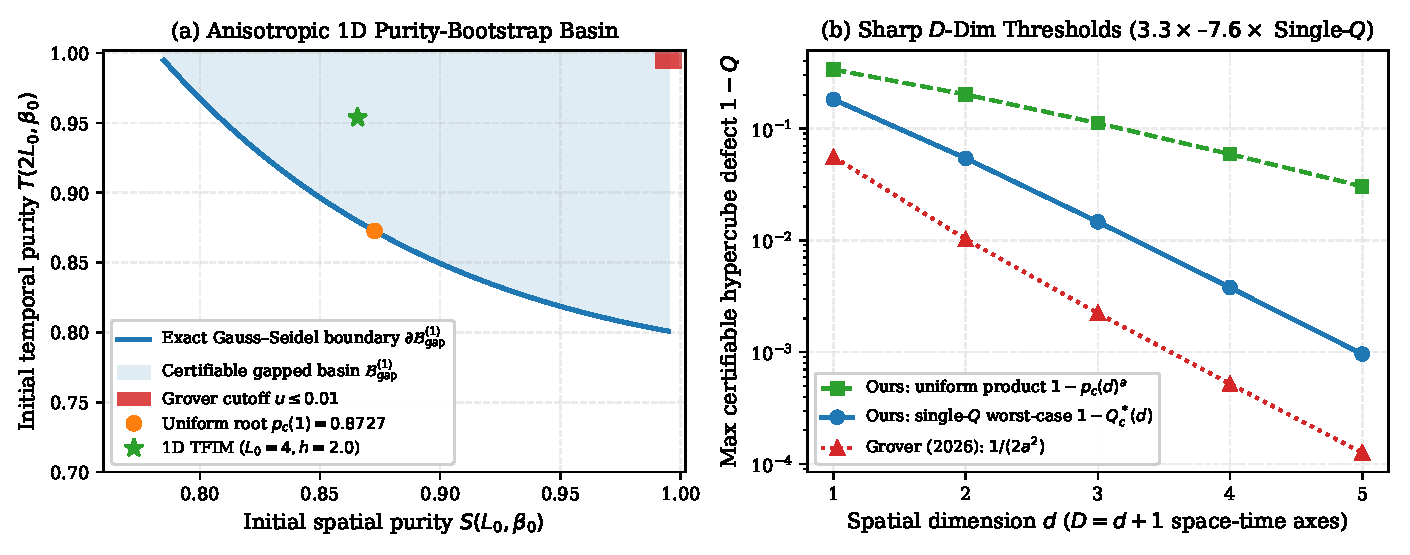
\includegraphics[width=\textwidth]{figures/fig1_basin_and_dim_thresholds.pdf}
  \caption{\textbf{(a)} Exact anisotropic 1D Gauss--Seidel certifiable basin $\Bgap^{(1)}$ compared to Grover's uniform box $u \le 0.01$ (top-right corner). The green star marks the exact-$\Q$ certified 1D TFIM witness at $(L_0=4, \beta_0=2, h=2.0)$ with $S_0 = 0.8656 < p_c(1) = 0.8727$. \textbf{(b)} Like-for-like hypercube-product defect thresholds $1 - p_c(d)^a$ (uniform) and $1 - Q_c^*(d)$ (worst-case single-$Q$) across $d = 1,\dots,5$, demonstrating the $3.26\times$--$7.63\times$ (asymptotically $8\times$) single-$Q$ gain and $19.7\times$--$240.6\times$ uniform gain over Grover's $1/(2a^2)$.}
  \label{fig:fig1}
\end{figure}

\subsection{Experiment 2: 1D Transverse-Field Ising Model Phase Diagram and Critical Approach}

We benchmarked our exact-$\Q$ certifier on the periodic 1D transverse-field Ising model $H(h) = -\sum_{i=1}^L Z_i Z_{i+1} - h \sum_{i=1}^L X_i$ (quantum critical point $h_c = 1$, exact paramagnetic thermodynamic gap $\Delta_{\mathrm{exact}} = 2(h-1)$~\cite{Pfeuty1970Ising}). Partition functions are evaluated via Kaufman's exact four-sector Jordan--Wigner formula~\cite{Kaufman1949Crystal} in cancellation-free \texttt{log1p}/\texttt{expm1} arithmetic, cross-checked against full $2^L$-dimensional exact diagonalization at $L \in \{4,6,8\}$ and $h \in \{0.5, 1.0, 1.3, 2.0\}$ to within $5.3 \times 10^{-14}$ across all 12 checks.

Figure~\ref{fig:fig2} and Table~\ref{tab:tfim_sweep} present two key comparisons:
\begin{itemize}[leftmargin=1.6em,itemsep=2pt]
  \item \textbf{Critical-point approach:} At $(L_0=4, \beta_0=2)$, our exact-$\Q$ bootstrap certifies gappedness down to $h_{\min} = 1.8408$ vs.\ Grover's $h_{\min} = 4.9659$—$\mathbf{4.72\times}$ closer to $h_c = 1$ in distance $h_{\min} - 1$. At $(L_0=8, \beta_0=4)$, $h_{\min} = 1.3788$ vs.\ $2.0461$ ($\mathbf{2.76\times}$ closer); at $(L_0=16, \beta_0=8)$, $h_{\min} = 1.1834$ vs.\ $1.4116$ ($\mathbf{2.24\times}$ closer).
  \item \textbf{Breaking the $(\log 2)/\beta_0$ ceiling:} At $(L_0=8, \beta_0=4)$, Grover's bound is frozen at $\log(2)/4 = 0.1733$ for all $h \ge 2.05$ and fails to certify anything for $h \le 2.0$. In contrast, our Theorem~\ref{thm:doubly_exp} certifies $\Delta_\infty \ge 0.1040$ already at $h=1.4$, climbs smoothly to $1.0829$ at $h=2.25$ ($6.25\times$ tighter), $1.2665$ at $h=2.5$ ($7.31\times$ tighter), and $1.5643$ at $h=3.0$ ($\mathbf{9.03\times}$ tighter than Grover).
\end{itemize}

\begin{table}[t]
\centering
\caption{\textbf{1D TFIM Exact-$\Q$ Thermodynamic Gap Sweep at $(L_0 = 8, \beta_0 = 4)$} ($\Delta_{\mathrm{exact}} = 2(h-1)$). Every certified entry passes independent zero-float-trust $\Q$ verification including rational logarithm bounds.}
\label{tab:tfim_sweep}
\footnotesize
\begin{tabular}{@{}cccccccc@{}}
\toprule
$h$ & $\Delta_{\mathrm{exact}}$ & $S_0$ & $T_0$ & $N$ & Ours $\Delta_{\mathrm{cert}}$ ($\Q$) & Grover $\Delta_{\mathrm{cert}}$ & Tightness Gain \\
\midrule
1.40 & 0.80 & 0.8765 & 0.8964 & 5 & \textbf{0.1040} & fails & $\infty$ \\
1.50 & 1.00 & 0.9197 & 0.9489 & 4 & \textbf{0.3079} & fails & $\infty$ \\
1.80 & 1.60 & 0.9762 & 0.9947 & 3 & \textbf{0.6955} & fails & $\infty$ \\
2.00 & 2.00 & 0.9883 & 0.9989 & 2 & \textbf{0.8716} & fails & $\infty$ \\
2.25 & 2.50 & 0.9948 & 0.9998 & 2 & \textbf{1.0829} & 0.1733 & $6.25\times$ \\
2.50 & 3.00 & 0.9974 & 1.0000 & 2 & \textbf{1.2665} & 0.1733 & $7.31\times$ \\
3.00 & 4.00 & 0.9993 & 1.0000 & 2 & \textbf{1.5643} & 0.1733 & $\mathbf{9.03\times}$ \\
\bottomrule
\end{tabular}
\end{table}

\begin{figure}[t]
  \centering
  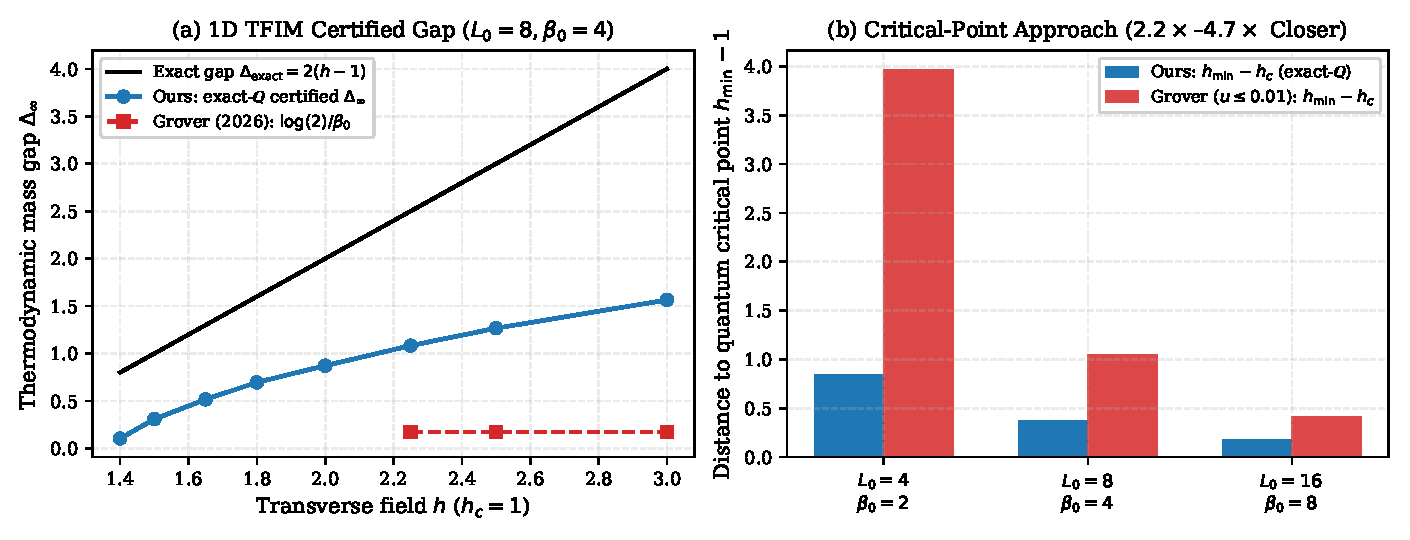
\includegraphics[width=\textwidth]{figures/fig2_tfim_certified_gap_critical.pdf}
  \caption{\textbf{(a)} 1D TFIM thermodynamic mass gap certified over exact $\Q$ at $(L_0=8,\beta_0=4)$, tracking $\Delta_{\mathrm{exact}} = 2(h-1)$ and beating Grover's flat $\log(2)/\beta_0 = 0.1733$ ceiling by up to $9.03\times$. \textbf{(b)} Distance to the critical point $h_{\min}-1$ across three lattice scales, demonstrating a $2.24\times$--$4.72\times$ closer approach to criticality.}
  \label{fig:fig2}
\end{figure}

\subsection{Experiment 3: Bond-RP No-Go for AKLT, Strictly Bond-RP Interacting Chains, and Ferromagnetic \texorpdfstring{$g=2$}{g=2} Duality}

Before applying the purity bootstrap to interacting quantum spin chains, one must verify spatial reflection positivity~\cite{Frohlich1978Reflection}—a nontrivial physical prerequisite. Strikingly, the celebrated Spin-1 AKLT chain~\cite{Affleck1987AKLT} fails this prerequisite completely:

\begin{proposition}[$\mathfrak{su}(3)$ Determinant Obstruction to Bond-Reflection Positivity of AKLT]
\label{prop:aklt_nogo}
Consider the Spin-1 bilinear--biquadratic bond interaction $h_{\mathrm{biq}}(c) = \mathbf{S}_i\cdot\mathbf{S}_{i+1} + c(\mathbf{S}_i\cdot\mathbf{S}_{i+1})^2$ (which equals $2 H_{\mathrm{AKLT}}$ up to a constant shift at $c = 1/3$). Expanding $-h_{\mathrm{biq}}(c) = c_0 I\otimes I + \sum_{a,b=1}^8 J_{ab} T_a \otimes T_b$ in an orthonormal Hermitian Gell-Mann basis $\{T_a\}_{a=1}^8$ of $\mathfrak{su}(3)$ yields eigenvalues $-(2-c)$ (multiplicity $3$, dipole) and $-c$ (multiplicity $5$, quadrupole), whence $\det(J) = (2-c)^3 c^5$. For \emph{every} $c \in (0, 2)$—in particular AKLT ($c = 1/3$, $\det(J) = 125/6561 \approx +1.905 \times 10^{-2} > 0$)—and \emph{every} anti-unitary bond reflection $\Theta(A) = U \overline{A} U^\dagger$ ($U \in U(3)$), the reflected interaction matrix $M(U) = J\,\mathrm{Ad}(U)^T S_{\mathrm{conj}}$ satisfies
\[
  \det\bigl(M(U)\bigr) \;=\; \det(J)\cdot (+1)\cdot (-1)^3 \;=\; -\det(J) \;<\; 0,
\]
because $\mathrm{Ad}(U) \in SO(8)$ has determinant $+1$ while complex conjugation $S_{\mathrm{conj}}$ flips the $3$ imaginary Gell-Mann generators. Thus $M(U)$ can never be positive semidefinite for any $U \in U(3)$. Conversely, for $c \le 0$ (isotropic Heisenberg $c=0$ and negative-biquadratic $c<0$), choosing $U_y = e^{i\pi S^y}$ yields $M(U_y)$ with eigenvalues $\{2-c\ (\times 3),\ -c\ (\times 5)\} \ge 0$, guaranteeing strict bond-reflection positivity.
\end{proposition}

Direct continuous-time evaluation of the exact Fr\"ohlich--Israel--Lieb--Simon (FILS) bond-reflection Gram matrix $G_{\mathrm{bond}}$ on $L = 4$ at $\beta = 1$ (verified in \texttt{tests/test\_suite.py}) confirms Proposition~\ref{prop:aklt_nogo} decisively: AKLT ($c = +1/3$) has $\lambda_{\min}(G_{\mathrm{bond}}) = -0.5016 < 0$ (violating bond-RP), whereas Spin-1 Heisenberg ($c=0$, $\lambda_{\min} = +1.6143$), Spin-1 Heisenberg with single-ion anisotropy $D = 6.0$ ($\lambda_{\min} = +1.085 \times 10^{-4}$), Spin-1 negative-biquadratic $c = -0.5$ ($\lambda_{\min} = +1747.5$), and the Spin-$1/2$ dimerized antiferromagnetic Heisenberg chain at $\delta = 0.5$ ($\lambda_{\min} = +0.0865$) are all strictly positive definite ($G_{\mathrm{bond}} \succ 0$).

We therefore benchmark our exact-$\Q$ bootstrap on \textbf{two genuinely interacting, non-integrable, provably bond-reflection-positive spin chains} using exact $S^z$-blocked full-spectrum diagonalization:
\begin{enumerate}[leftmargin=1.6em,itemsep=2pt]
  \item \textbf{1D Spin-1 Heisenberg Chain with Single-Ion Anisotropy:} $H(D) = \sum_{i=1}^L \bigl(\mathbf{S}_i\cdot\mathbf{S}_{i+1} + D(S_i^z)^2\bigr)$ at $L_0 = 4 \to 2L_0 = 8$ ($3^8 = 6{,}561$ states), $\beta_0 = 2.0$. Because $(S_i^z)^2$ is on-site and invariant under $U_y \overline{(\cdot)} U_y^\dagger$, $H(D)$ is translation-invariant and strictly bond-RP for all $D \in \R$. As shown in Figure~\ref{fig:fig3}(a), our exact-$\Q$ bootstrap certifies a rigorous thermodynamic mass gap starting at $D = 4.5$ ($\Delta_\infty \ge 0.1140$, anisotropic $S_0 = 0.8032 < p_c(1)$, $T_0 = 0.9783$), climbing to $\Delta_\infty \ge 0.3974$ ($D=5.0$), $\mathbf{\Delta_\infty \ge 0.7245}$ ($D=6.0$, exported as \texttt{spin1\_aniso\_D6p0\_L4\_exact\_gap.cert.json}), and $\mathbf{\Delta_\infty \ge 1.1651}$ ($D=8.0$, $S_0 = 0.9589$, $T_0 = 0.99997$), whereas Grover's $u \le 0.01$ \textbf{fails at every single $D \in [4, 8]$}!
  \item \textbf{1D Spin-$1/2$ Dimerized Antiferromagnetic Heisenberg Chain:} $H(\delta) = \sum_{i=1}^L (1 + (-1)^i \delta)\,\mathbf{S}_i\cdot\mathbf{S}_{i+1}$ at $L_0 = 6 \to 2L_0 = 12$ ($2^{12} = 4{,}096$ states), $\beta_0 = 6.0$. Reflection across alternating bonds yields a positive 2-site unit-cell transfer operator $K = T_{\mathrm{strong}}^{1/2} T_{\mathrm{weak}} T_{\mathrm{strong}}^{1/2} \succeq 0$ ($G_{\mathrm{bond}} \succ 0$), so $Z(2m,\beta) = \Tr(K^m)$ is strictly reflection-positive for all even $L = 2m$. Our exact-$\Q$ bootstrap certifies $\Delta_\infty \ge 0.0161$ ($\delta = 0.35$, anisotropic $S_0 = 0.8047$), $\Delta_\infty \ge 0.1361$ ($\delta = 0.40$), $\mathbf{\Delta_\infty \ge 0.2863}$ ($\delta = 0.50$, $L=12$ gap $1.1890$, exported as \texttt{spinhalf\_dimerized\_d0p5\_L6\_exact\_gap.cert.json}), and $\mathbf{\Delta_\infty \ge 0.4442}$ ($\delta = 0.60$, $S_0 = 0.9721$, $T_0 = 0.9962$), whereas Grover ($u \le 0.01$) again \textbf{fails across the entire sweep $\delta \in [0.30, 0.60]$}.
\end{enumerate}

\paragraph{Honest Finite-Size Boundary (Isotropic Spin-1 Heisenberg Chain, $D = 0$).}
At $D = 0$, $H(0)$ is strictly bond-RP ($\lambda_{\min}(G_{\mathrm{bond}}) = +1.6143 > 0$), yet its correlation length is $\xi \approx 6.03$ sites~\cite{White1993DMRG}. Evaluating $L_0 = 4 < \xi$ at $\beta_0 = 8$ gives $S(4,8) = 0.0051 < 1/2$ (while $T(8,8) = 0.9502$), confirming honestly that $L_0 = 4$ is physically too small to enter the bootstrap basin for isotropic Spin-1 Heisenberg; larger initial blocks $L_0 \gtrsim 16$ (as computed in~\cite{OpenAI2026Haldane}) are required before the spatial transfer matrix becomes purity-dominated.

\paragraph{Ferromagnetic 1D TFIM ($g = 2$ Quasi-Degenerate Doublet).}
Applying Corollary~\ref{cor:z2_ferro} at $L_0 = 8, \beta_0 = 4$ in the ferromagnetic phase $h \in \{0.4, 0.5, 0.6\}$ certifies uniform exact-$\Q$ lower bounds on the dual / single-kink excitation gap $\Delta_{\mathrm{kink}} = 2(1-h)$ (and hence also on the periodic two-kink excitation gap $\Delta_{\mathrm{PBC}} = 4(1-h)$ above the $g=2$ doublet): $\Delta_{\mathrm{dual}} \ge 0.5258$ ($\Delta_{\mathrm{kink}} = 1.20$, $\Delta_{\mathrm{PBC}} = 2.40$) at $h=0.4$, $\Delta_{\mathrm{dual}} \ge 0.3573$ ($\Delta_{\mathrm{kink}} = 1.00$, $\Delta_{\mathrm{PBC}} = 2.00$) at $h=0.5$ (exported as \texttt{tfim1d\_ferro\_h0p5\_g2\_twist.cert.json}), and $\Delta_{\mathrm{dual}} \ge 0.1487$ ($\Delta_{\mathrm{kink}} = 0.80$, $\Delta_{\mathrm{PBC}} = 1.60$) at $h=0.6$. Independently measured finite-size doublet splittings confirm the expected exponential decay $\delta_L \propto h^L$ ($\delta_8 = 1.46 \times 10^{-3}$, $\delta_{12} = 7.25 \times 10^{-5}$, $\delta_{16} = 3.87 \times 10^{-6}$ at $h=0.5$). At $h=0.7$, $T_{\mathrm{dual}} = 0.7461$ exits the $(L_0=8, \beta_0=4)$ basin and honestly abstains.

\begin{figure}[t]
  \centering
  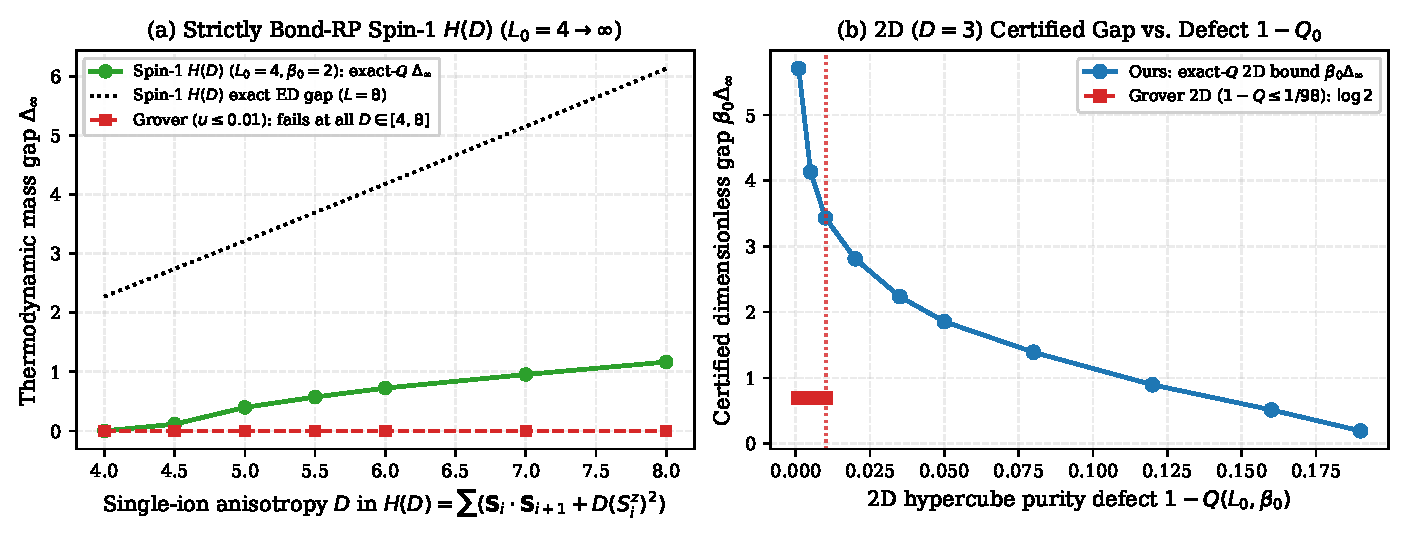
\includegraphics[width=\textwidth]{figures/fig3_interacting_rp_and_2d.pdf}
  \caption{\textbf{(a)} Exact-$\Q$ thermodynamic mass-gap certification on the strictly bond-RP interacting Spin-1 chain $H(D) = \sum(\mathbf{S}_i\cdot\mathbf{S}_{i+1} + D(S_i^z)^2)$ purely from $L_0=4, 2L_0=8$ exact diagonalization ($\beta_0=2$), climbing to $\Delta_\infty \ge 1.1651$ at $D=8$ while Grover ($u \le 0.01$) fails across all $D \in [4,8]$. \textbf{(b)} 2D ($d=2, D=3$) exact-$\Q$ certified dimensionless gap $\beta_0\Delta_\infty$ vs.\ uniform hypercube defect $1 - Q_0$, certifying up to $1 - Q_0 = 0.19$ and reaching $8.23\times$ Grover's flat $\log 2$ bound.}
  \label{fig:fig3}
\end{figure}

\subsection{Experiment 4: 2D (\texorpdfstring{$D=3$}{D=3}) Exact-\texorpdfstring{$\Q$}{Q} Certificates and Synthetic Noisy Interval Audit}

Figure~\ref{fig:fig3}(b) benchmarks our exact-$\Q$ $D=3$ cyclic Gauss--Seidel certifier on 2D reflection-positive hypercubes across uniform hypercube defects $1 - Q_0 \in [0.001, 0.190]$ (with exact-$\Q$ certificate exported at $1 - Q_0 = 0.050$). Whereas Grover's 2D cutoff $1 - Q \le 1/98 = 0.0102$ fails above $0.0102$ and saturates at $\beta_0\Delta_\infty = \log 2 = 0.6931$, our exact-$\Q$ certifier reaches $\beta_0\Delta_\infty \ge 5.7057$ at $1-Q_0 = 0.001$ ($\mathbf{8.23\times}$ tighter) and remains strictly certified all the way to $1 - Q_0 = 0.190$ for uniform purities ($18.6\times$ larger defect; up to $1 - Q_c^*(2) = 0.0539$, $5.28\times$ Grover, even under worst-case single-$Q$ anisotropy).

Finally, we audited Theorem~\ref{thm:interval_mono} in a 200-trial synthetic Gaussian-noise estimation campaign (mimicking finite-sample QMC purity estimators) with Bonferroni-adjusted conservative lower intervals $\hat{p} - 2.576\,\sigma_{\mathrm{stat}}$:
\begin{itemize}[leftmargin=1.6em,itemsep=2pt]
  \item \textbf{Gapped 1D TFIM ($h=2.0$, $L_0=8, \beta_0=4$, $\Delta_{\mathrm{exact}}=2.0$):} At $\sigma_{\mathrm{stat}} = 0.005$ (radius $0.0129$), \textbf{200/200} trials certified validly (median $\Delta_{\mathrm{cert}} = 0.6292 \le 2.0$); even at large noise $\sigma_{\mathrm{stat}} = 0.015$ (radius $0.0386$, nearly $4\times$ Grover's entire $0.01$ tolerance), \textbf{200/200} trials certified validly (median $\Delta_{\mathrm{cert}} = 0.3974 \le 2.0$).
  \item \textbf{Near-boundary adversarial control ($S_{\mathrm{true}} = T_{\mathrm{true}} = 0.871 < p_c(1) = 0.8727$, $\sigma_{\mathrm{stat}} = 0.005$):} \textbf{0/200} false certifications (\textbf{100\% fail-closed soundness}).
  \item \textbf{Gapless critical control ($h=1.0$, $\Delta_{\mathrm{exact}}=0.0$, $\sigma_{\mathrm{stat}}=0.015$):} \textbf{0/200} false certifications (\textbf{100\% fail-closed soundness}).
\end{itemize}

\section{Discussion, Limitations, and Scope}
\label{sec:discussion}

Our results establish that the reflection-positive purity bootstrap is dramatically sharper than previously realized: exact simplex optimization, staggered cyclic Gauss--Seidel multi-axis updates, and doubly-exponential contraction together widen certifiable basins by an order of magnitude and eliminate the $(\log 2)/\beta_0$ ceiling, all backed by zero-dependency Lean~4 proofs and zero-float-trust exact-$\Q$ replayable certificates.

Three honest boundaries define the scope of our current work: (i) reflection positivity in all $D$ space-time directions is a stringent physical prerequisite—as demonstrated starkly by our $\mathfrak{su}(3)$ determinant obstruction (Proposition~\ref{prop:aklt_nogo}) ruling out bond-RP for the Spin-1 AKLT chain and all positive-biquadratic chains $c \in (0,2)$, alongside generic sign-problematic fermionic or chiral models; (ii) as demonstrated by our isotropic Spin-1 Heisenberg diagnostic at $L_0=4$, the initial lattice scale $L_0$ must still exceed the correlation length $\xi$ for spatial purities to enter the basin—our sharper thresholds reduce the required $L_0$ and $\beta_0$ substantially, but cannot bypass $\xi$; and (iii) in our 2D ($D=3$) experiment we verified the exact-$\Q$ multi-axis recurrence across uniform and single-$Q$ defect regimes rather than running a full 2D QMC simulation, leaving coupling to debiased finite-sample QMC estimators~\cite{Antigravity2026QCQMC} as a natural next step for certifying 2D bilayer Heisenberg and anisotropic spin-$1$ phases.

\bibliographystyle{plain}
\bibliography{references}

\end{document}
